
\documentclass{scrartcl}
\usepackage{tikz}
\usetikzlibrary{arrows,automata}

\begin{document}
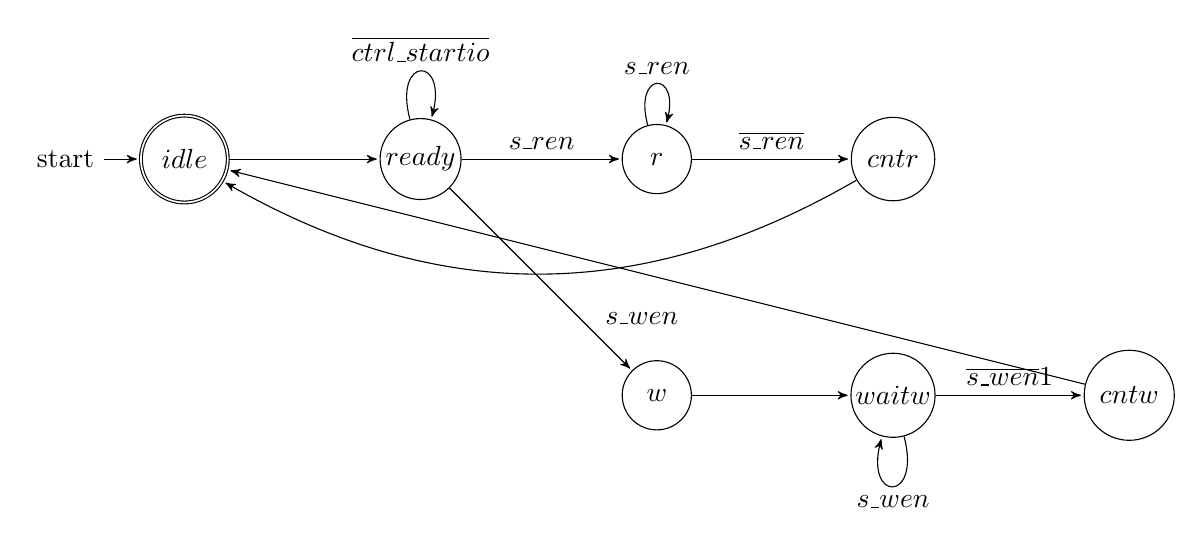
\begin{tikzpicture}[>=stealth',shorten >=1pt,auto,node distance=3cm]
  \node[initial,state,accepting, inner sep=5pt] (idle)   {$idle$};
  \node[state, inner sep=1pt]                   (ready) [right of=idle]  {$ready$};
  \node[state, inner sep=5pt]                   (r)     [right of=ready] {$r$};
  \node[state, inner sep=5pt]                   (w)     [below of=r]     {$w$};
  \node[state, inner sep=4pt]                   (cntr)  [right of=r]     {$cntr$};
  \node[state, inner sep=1pt]                   (waitw) [right of=w]     {$waitw$};
  \node[state, inner sep=4pt]                   (cntw)  [right of=waitw] {$cntw$};


  \path[->]
  (idle)
  edge
  node [loop above]
  {} (ready)

  (ready)
  edge 
  node
  {$s\_ren$} (r)
  edge [pos=0.8] 
  node
  {$s\_wen$} (w)
  edge [loop above] 
  node
  {$\overline{ctrl\_startio}$} (ready)

  (w)
  edge 
  node
  {} (waitw)

  (r)
  edge [loop above]
  node
  {$s\_ren$} (r)
  edge 
  node
  {$\overline{s\_ren}$} (cntr)

  (waitw)
  edge [loop below]
  node
  {$s\_wen$} (cntw)
  edge 
  node
  {$\overline{s\_wen}$1} (cntw)

  (cntr)
  edge [bend left]
  node
  {} (idle)

  (cntw)
  edge 
  node
  {} (idle)
;



\end{tikzpicture}
\end{document}
